
%使用XeLaTeX编译
%版权所有,翻版必究
%本文件由程序自动生成,任何修改将被覆盖
%2019 年 01 月 23 日





由于Qt Quick的所有渲染最终都
依靠现代3D可编程渲染管线实现。
这样读者就可以
在原有管线的基础上任意添加
新的渲染管线。

毫无疑问,读者可以不受限的将
所有现代渲染技术应用到
应用程序之中。

对于常见图形特效,Qt Quick
提供了“Qt Graphical Effects”
模块。

本章将带领读者纵览
Qt Graphical Effects提供的
25种图形特效。

\FloatBarrier
\section{
导引
}\label{c000015s000001}


%begin图片
\begin{figure}[htb] %浮动体 here and top ...
%there must use marginnote ...
\marginnote{\setlength\fboxsep{2pt}\fbox{\footnotesize{\kaishu\figurename\,}\footnotesize{\ref{p000012}}}}\centering %中心对齐
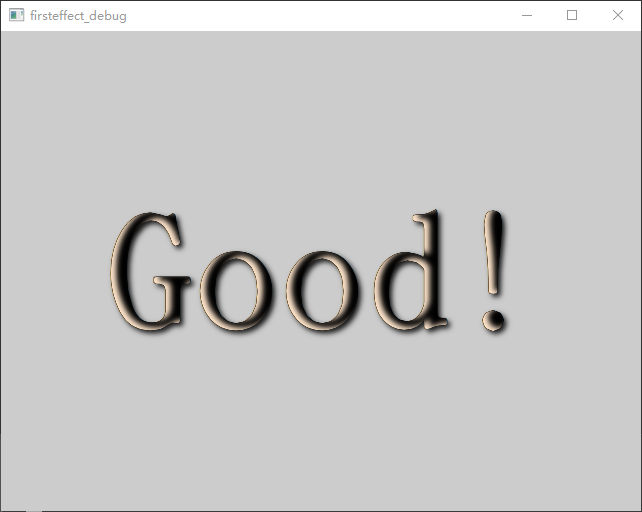
\includegraphics[width=0.95\textwidth]{../chapter06/firsteffect/the_app.png} %图片路径
\caption{文字阴影} %标题
\label{p000012} %索引
\end{figure}
%end图片


要使用Qt Graphical Effects
只需要在Qml文件开头增加一行:\\
import QtGraphicalEffects 1.12

\filesourcenumbernameone\ \ref{f000051}展示了
使用“DropShadow”和“InnerShadow”模拟光照,
虚拟立体文字。

值得注意的是,
图形特效不应当是其源(source)对象的子对象。
否则,上一次图形特效渲染出的结果会加入下一次运算。
这会造成渲染出现闭环。
在绝大多数情况下这种闭环会导致错误的渲染结果。

%\begin{spacing}{1.0}
\refstepcounter{filesourcenumber}\label{f000051}    %增加源代码编号
\FloatBarrier                                  %强制完成浮动体布局
\begin{thebookfilesourceone}[escapeinside={(*@}{@*)},
caption=GoodLuck,
title=\filesourcenumbernameone \thefilesourcenumber
]
/*firsteffect/main.qml*/
import QtQuick 2.9
import QtGraphicalEffects 1.12

Rectangle {

    id : idRoot
    width: 640;
    height: 480;
    color: Qt.rgba(0.8,0.8,0.8,1);

    RenderText{
        id : idText
        text: "Good!"
        font.pointSize: 128
        font.bold: true
        anchors.centerIn: parent
        color: Qt.darker( idInnerShadow.color ) ;
    }

    DropShadow{
        anchors.fill: idText
        horizontalOffset: 3
        verticalOffset: 3
        radius: 8.0
        samples: 17
        color: Qt.rgba(0.1,0.1,0.1,1)
        source: idText
    }

    InnerShadow{
        id : idInnerShadow
        anchors.fill: idText
        radius: 8.0
        samples: 16
        horizontalOffset: 5.5
        verticalOffset: -2.8
        color: Qt.rgba(1,0.9,0.8,1)
        source: idText
    }

}/*~Rectangle*/(*@\marginpar[\hfill\setlength\fboxsep{2pt}\fbox{\footnotesize{\kaishu\parbox{1em}{\setlength{\baselineskip}{2pt}\filesourcenumbernameone}}\footnotesize{\thefilesourcenumber}}]{\setlength\fboxsep{2pt}\fbox{\footnotesize{\kaishu\parbox{1em}{\setlength{\baselineskip}{2pt}\filesourcenumbernameone}}\footnotesize{\thefilesourcenumber}}}@*)\end{thebookfilesourceone}          %抄录环境
\addtocounter{lstlisting}{-1}   %sub lstlisting counter ...
%\end{spacing}


Qt Graphical Effects共提供了25种图形特效,
如\tablename\ \ref{tb000000}所示:


%使用XeLaTeX编译
%版权所有,翻版必究
%本文件由程序自动生成,任何修改将被覆盖
%2019 年 01 月 23 日



%表
\begin{longtable}{ccc}

%表头....
\toprule{}类名 
&
分类
&
简介%there must use marginnote ...
\marginnote{\setlength\fboxsep{2pt}\fbox{\footnotesize{\kaishu\tablename\,}\footnotesize{\ref{tb000000}}}}
\\ \midrule 
\endfirsthead

%表尾...
\bottomrule
\caption{ThresholdMask}\label{tb000000} 
\endlastfoot

%重复表头
\toprule{}类名 
&
分类
&
简介
\\ \midrule
\endhead
%重复表尾
\midrule
\endfoot 
Blend & aabbc & cccc \\
BrightnessContrast & aabbc & cccc \\
ColorOverlay & aabbc & cccc \\
Colorize & aabbc & cccc \\
Desaturate & aabbc & cccc \\
GammaAdjust & aabbc & cccc \\
HueSaturation & aabbc & cccc \\
LevelAdjust & aabbc & cccc \\
ConicalGradient & aabbc & cccc \\
LinearGradient & aabbc & cccc \\
RadialGradient & aabbc & cccc \\
Displace & aabbc & cccc \\
DropShadow & aabbc & cccc \\
InnerShadow & aabbc & cccc \\
FastBlur & aabbc & cccc \\
GaussianBlur & aabbc & cccc \\
MaskedBlur & aabbc & cccc \\
RecursiveBlur & aabbc & cccc \\
DirectionalBlur & aabbc & cccc \\
RadialBlur & aabbc & cccc \\
ZoomBlur & aabbc & cccc \\
Glow & aabbc & cccc \\
RectangularGlow & aabbc & cccc \\
OpacityMask & aabbc & cccc \\
ThresholdMask  & aabbc & cccc \\
\end{longtable}
%表





%使用XeLaTeX编译
%版权所有,翻版必究
%本文件由程序自动生成,任何修改将被覆盖
%2019 年 01 月 23 日














%使用XeLaTeX编译
%版权所有,翻版必究
%本文件由程序自动生成,任何修改将被覆盖
%2019 年 01 月 23 日



